\section{Problema 3: El se\~nor de los caballos}
\subsection{Descripci\'on de la problem\'atica}

En este problema, se presenta un tablero de ajedrez de tama\~no $nxn$, el cual cuenta con alguna cantidad de caballos ubicados en una posici\'on aleatoria del tablero. Lo que se quiere lograr es \emph{cubrir} todo el tablero. Un casillero se considera cubierto si hay un caballo en \'el o bien, si es una posici\'on en la cual alg\'un caballo existente puede moverse con un s\'olo movimiento. Para lograr este cometido, puede ser necesario agregar nuevas fichas \emph{caballo} al tablero. No existe un l\'imite en la cantidad de caballos para agregar, pero lo que se busca es dar una soluci\'on con la m\'inima cantidad de caballos posibles.\\


En la figura \ref{caballito} se pueden ver todas las casillas que est\'an cubiertas por un s\'olo caballo.


% \begin{figure}[h!]
%   \begin{center}
% 	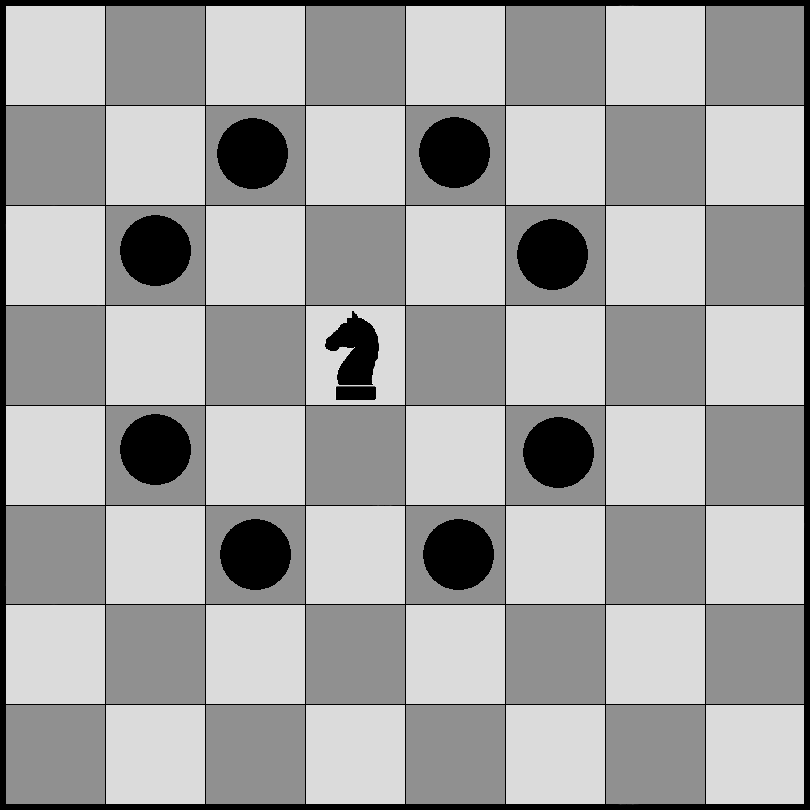
\includegraphics[scale=0.3]{imagenes/ej3/caballito.png}
% 	\caption{Casillas que \emph{cubre} un caballo}
% 	\label{caballito}	
%   \end{center}
% \end{figure}



\newpage
\subsection{Resoluci\'on propuesta y justificaci\'on}
\textcolor{blue}{Esto va en algun lado?}\\
\textcolor{blue}{Ya no se ni donde van las cosas! JAJAJA}\\

Para la resoluci\'on de este ejercicio, se ped\'ia un algoritmo de backtracking. La soluci\'on que presentamos tiene inclu\'idas estrategias para que el algoritmo resuelva en un tiempo razonable los problemas medianos.\\

Vale aclarar que si el tablero ya estaba cubierto de antemano, simplemente hab\'ia que chequearlo, tomando $O(n^{2})$.\\

En primera instancia decidimos armar un algoritmo de backtracking "bobo", que revise todas las posibles combinaciones de tableros y nos devuelve la m\'as \'optima para este problema.\\

Simplemente se fija cu\'antos caballos necesita colocar para cubrir el tablero si no coloca un caballo en alguna posici\'on y luego se fija cu\'antos har\'an falta si lo pone en la misma posici\'on. Este m\'etodo de "fuerza bruta" tiene una complejidad de $O(2^{n^{2} - k})$ siendo n la dimensi\'on del tablero y k la cantidad de caballos preubicados. Esto es para cada posici\'on sin caballos, ver que pasa si tomo alguna de las dos posibles decisiones.\\

Para disminuir la cota de complejidad, se plantearon podas y estrategias, es decir, determinar si vale la pena o no seguir revisando alguna rama del \'arbol de soluciones que propone esta t\'ecnica de programaci\'on.\\

La primera poda fue la m\'as intuitiva, si tenemos una soluci\'on con k caballos extra agregados,  y analizando otra rama llegamos a tener que necesitar agregar un caballo a una subsoluci\'on de k-1 caballos (o sea que tendr\'ia k caballos), entonces no nos interesa seguir revisandola, pues tenemos una soluci\'on que es igual o m\'as \'optima con k caballos.\\

\textcolor{blue}{SHAMUSHO}\\

La segunda estrategia fue plantear si en alg\'un momento sab\'iamos que deb\'iamos agregar o no un caballo en un determinado casillero. Entonces, salteamos las k posiciones de los caballos preubicados y adem\'as salteamos aquellas posiciones que, estando atacadas, si le pusieramos un caballo, estar\'ian atancando a casilleros que ya est\'an siendo atacados por otros caballos.\\

\newpage

\subsection{An\'alisis de la complejidad}
\newpage

\subsection{C\'odigo fuente}
\newpage
\subsection{Experimentaci\'on}

\subsubsection{Constrastaci\'on Emp\'irica de la complejidad}
-Hacer lo que hicieron en clase\\
\newpage
